\documentclass[12pt, oneside]{article}
 
\usepackage{graphicx}
\usepackage{hyperref}
\graphicspath{ {../Images/} }

\begin{document}
\thispagestyle{empty}
\begin{center}
\begin{minipage}{0.9\linewidth}
    \centering


    {\normalsize Project Tender\par}
    \vspace{1cm}
    {\Large Project: Eavesdropping Protection In Conclave\par}
{\normalsize Client: CSIR\par}
    \vspace{1cm}
   {\Large Team: Team Name\par}
    {\normalsize Renaldo van Dyk (12204359)\par}
    {\normalsize Johann Dian Marx (12105202)\par}
    {\normalsize Sean Thomas Hill (12221458)\par}
    {\normalsize Andreas du Preez (12207871)\par}
    {\normalsize Shaun Meintjes (13310896)\par}
{\normalsize Department of Computer Science, University of Pretoria\par}
    \vspace{1cm}

 {\normalsize Date: May 2015}
\vspace{1cm}
    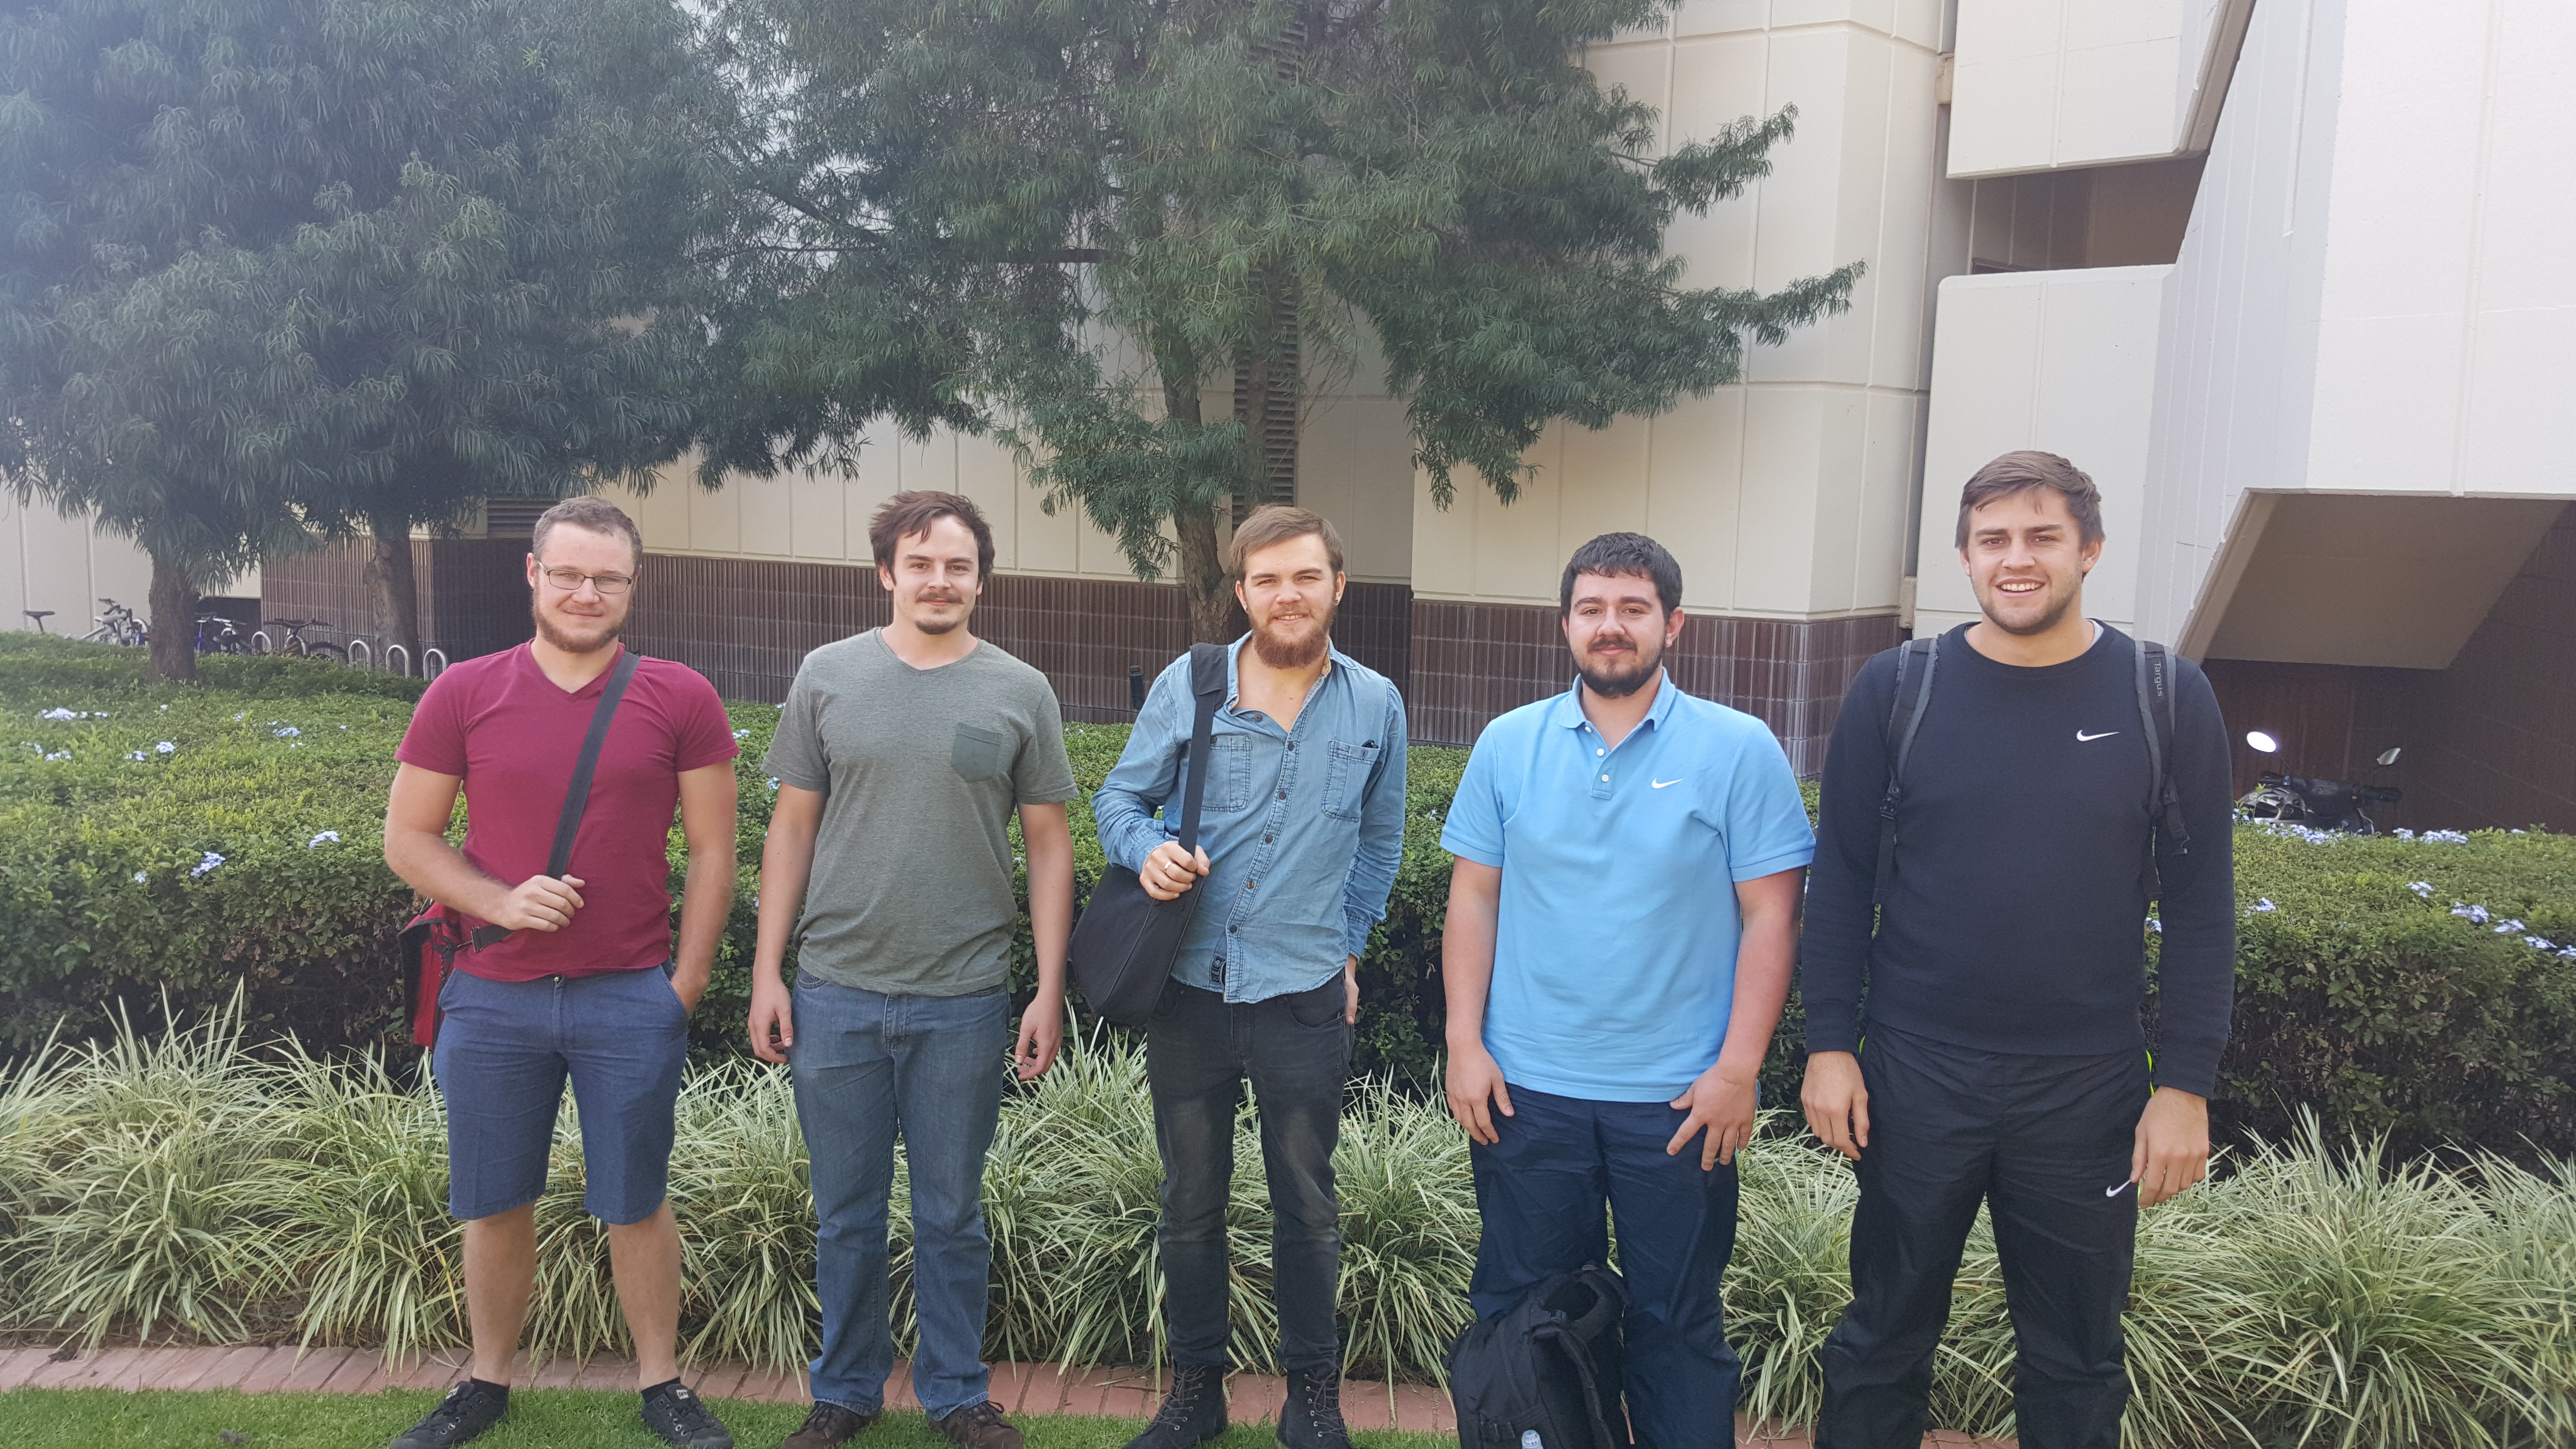
\includegraphics[scale=0.9]{example1} %Example is the name of the image

    \vspace{1cm}
    
\end{minipage}
\end{center}
\clearpage

\newpage

\section{The Team}
	\begin{enumerate}
		\item {Renaldo van Dyk (12204359)\par}
			
		\begin{itemize}		
			\includegraphics[scale=0.1]{Renaldo} %Example is the name of the image		
			\item Interests\newline\newline
				I'm a lover of technology in general and fortunate enough to pertain to it's value. I love knowing that 
				every page of code that I write will help improve someone in their day-to-day life. I mostly favour web and 
				mobile app development and I'm also intruiged by security and privacy aspects of information technology.\newline
			\item My technical strong points:
				\begin{itemize}
				\item Java\newline
					Java programming is one of my strong points and I have been using the java language extensively for 3 years.
				\item XML\newline
					XML have been used throughout the course of 4 years in my degree. We have learned how to use it 
					in different environments and I have experimented with it in my own time by writing small android apps.
				\item Web Technologies\newline
					PHP, Javascript, HTML, JQuery, AJAX, XML are some of my well developed skills.
				\item Other Languages\newline
					Visual C\#\newline
					C++\newline
					C\newline
					ASP.net\newline
					SQL\newline
					UML\newline	
				\end{itemize}				
			\item Past experience relevant to project\newline\newline
				I have worked on small Android apps, experimenting with some functionality including Wi-Fi, GEO location, voice recording etc. in order to get familiar with the Android SDK. The core of Android development lies in Java and XML. I have studied these languages to a great extent. This will make it easier for me to implement the mobile application and mobile malware.  I have worked with web technologies for 5 years, in my field of study and in the more corporate environment. This experience will be crucial in the development of the web server application.\newline
			\item Non-technical strengths\newline\newline
				I am  a strong perfectionist, this means I will not attemp a project if I am not 100\% sure that I will succeed. I am driven and always do my utmost best to reach deadlines.  Some of my charactaristics include:\newline 
Reliable\newline
Leader\newline
Precise\newline
Hard Working\newline
Passionate\newline
Loyal\newline
			\item What makes you want to do the project\newline\newline
				I love working with mobile development and web development and this project has a mixture of both. The fact that I have to write a malware application to test the mobile application intruiges me. This project can be used in big corporate companies and can be used on my resume.\newline
		\end{itemize}
		\item {Johann Dian Marx (12105202)\par}
		\begin{itemize}
			\item Photo\newline
				\includegraphics[scale=0.1]{example} %Example is the name of the image
			\item Interests\newline
				Fill in later...
			\item Technical Skills\newline
				Fill in later...
			\item Past experience relevant to project\newline
				Fill in later...
			\item Non-technical strengths\newline
				Fill in later...
			\item What makes you want to do the project\newline
				Fill in later...
		\end{itemize}
		\item {Sean Thomas Hill (12221458)\par}
		\begin{itemize}
			\item Photo\newline
				\includegraphics[scale=0.1]{example} %Example is the name of the image
			\item Interests\newline
				Fill in later...
			\item Technical Skills\newline
				Fill in later...
			\item Past experience relevant to project\newline
				Fill in later...
			\item Non-technical strengths\newline
				Fill in later...
			\item What makes you want to do the project\newline
				Fill in later...
		\end{itemize}
		\item {Andreas du Preez (12207871)\par}
		\begin{itemize}
			\item Photo\newline
				\includegraphics[scale=0.1]{example} %Example is the name of the image
			\item Interests\newline
				Fill in later...
			\item Technical Skills\newline
				Fill in later...
			\item Past experience relevant to project\newline
				Fill in later...
			\item Non-technical strengths\newline
				Fill in later...
			\item What makes you want to do the project\newline
				Fill in later...
		\end{itemize}
		\item {Shaun Meintjes (13310896)\par}
		\begin{itemize}
				\includegraphics[scale=0.1]{Shaun} %Example is the name of the image
			\item Interests\newline
				I have an interest in technology and new software that makes our daily lives easier and fun. I love to 						develop and create new things. I enjoy a challenge and then succeeding in the end. I enjoy web and 						mobile development, as well as writing systems for statistics and finances.
			\item Technical Skills\newline
				\begin{itemize}
				\item {\bf Java}\newline
					Java is the language I enjoy most. I have been using Java for the past 4 years.
				\item {\bf XML}\newline
					I have used XML during my degree, and I have learned how to use it effectively.
				\item {\bf Web Technologies}\newline
					PHP, Javascript, HTML, JQuery, AJAX, XML are some of the skills that I have acquired.
				\item {\bf Other Languages}\newline
					Visual C\#\newline
					C++\newline
					C\newline
					SQL\newline
					UML\newline	
					Fortran\newline
					COBOL\newline
					Assembly\newline
				\end{itemize}
			\item Past experience relevant to project\newline
				Fill in later...
			\item Non-technical strengths\newline
				Fill in later...
			\item What makes you want to do the project\newline
				Fill in later...
		\end{itemize}
	\end{enumerate}
	
\section{Project Execution}
	\subsection{Development Methodology}
		Fill in later...
	\subsection{How to keep the client informed about the status of the project}
		Fill in later...
	\subsection{Initial ideas on solving some of the technical challenges}
		Fill in later...
	\subsection{Techologies we intend to use for the project}
		Fill in later...
	\subsection{What the client will receive from us at the end of the project}
		Fill in later...
	\subsection{Etc.}
		Fill in later...

\end{document}